% $Id: Attribute_obj.tex,v 1.1 2008/02/26 03:29:22 rokuingh Exp $
%
% Earth System Modeling Framework
% Copyright 2002-2007, University Corporation for Atmospheric Research,
% Massachusetts Institute of Technology, Geophysical Fluid Dynamics
% Laboratory, University of Michigan, National Centers for Environmental
% Prediction, Los Alamos National Laboratory, Argonne National Laboratory,
% NASA Goddard Space Flight Center.
% Licensed under the University of Illinois-NCSA License.

\subsection{Object Model}

The following is a simplified UML diagram showing the structure of the
Attribute class.  See Appendix A, {\it A Brief Introduction to UML},
for a translation table that lists the symbols in the diagram and their 
meaning.

%\begin{center}
%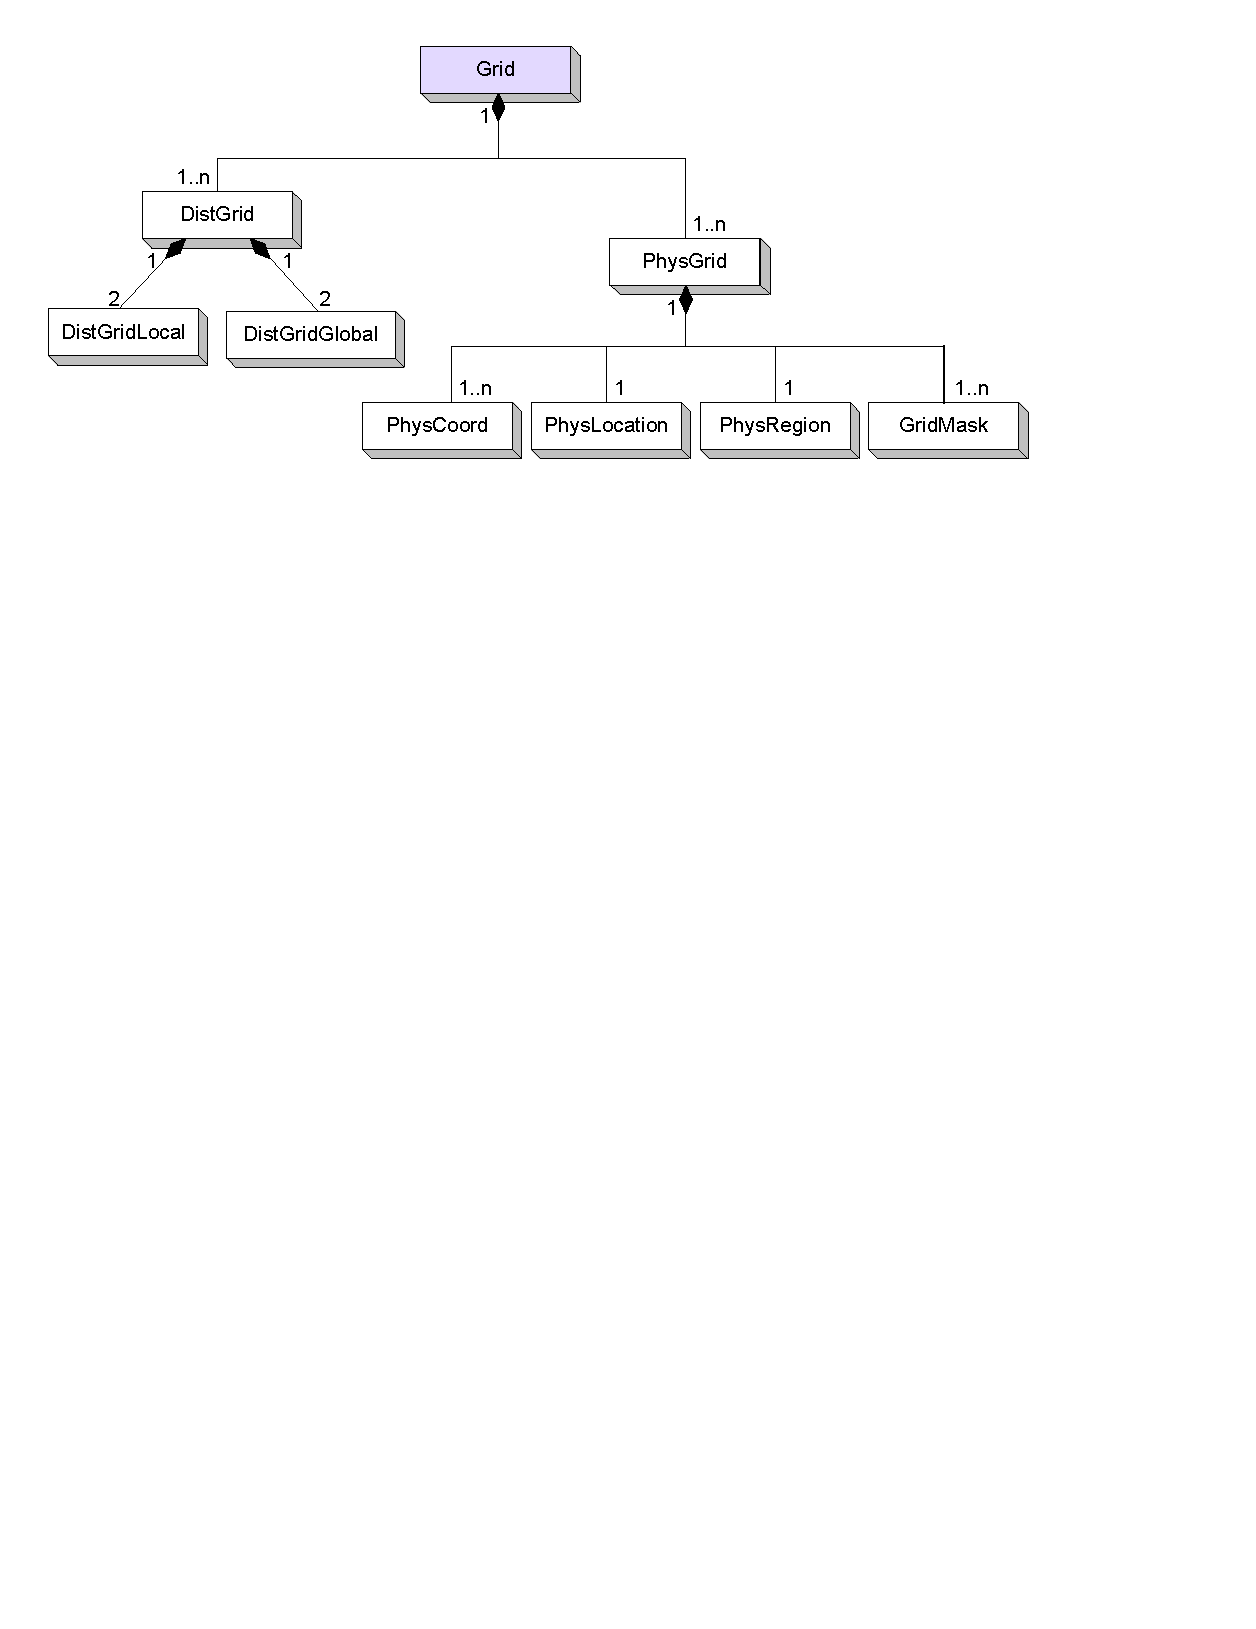
\includegraphics{Grid_obj}   
%\end{center}

Each Attribute contains a name value pair in which the value can be any of several numeric, character, and logical types.  All Attributes also contain character strings specifying the convention, type, and object of the Attribute for the purpose of keeping track of attribute packages.  All Attributes contain a pointer to a list of pointers to other Attributes, which is initialized as ESMF_NULL until specified otherwise.

